\section{Capítulo 5 -- Árvores}

Listas, pilhas e filas são estruturas \textbf{lineares}: cada elemento tem, no máximo, um anterior e um seguinte. Muitos dados do mundo real, porém, não são assim. As pastas do seu computador, o organograma de uma empresa e a estrutura de uma página HTML são \textbf{hierárquicos}: um item contém outros, que contêm outros. Neste capítulo você vai estudar a estrutura que representa hierarquias, a \textbf{árvore}, e uma de suas versões mais úteis, a \textbf{árvore binária de busca}, que permite procurar um valor entre milhões em poucas comparações.

\subsection{5.1 Organização hierárquica}

Uma árvore é formada por \textbf{nós} ligados por \textbf{arestas}. Existe um nó especial no topo, a \textbf{raiz}, e cada um dos outros nós tem exatamente um nó acima dele. Diferente das árvores da natureza, na computação a raiz é desenhada em cima e a árvore cresce para baixo.

Um bom exemplo é a expressão $(3 + 5) \cdot 4 - 2$. O operador que é calculado por último, o $-$, fica na raiz; seus dois operandos ficam abaixo dele, e assim por diante, até os números, que ficam nas pontas:

\begin{center}
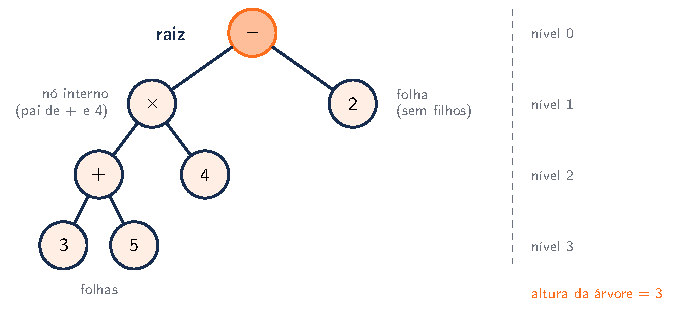
\includegraphics[width=0.85\linewidth,keepaspectratio]{imagens/capitulo-05_termos.pdf}
\end{center}

Repare que os parênteses desapareceram: a própria forma da árvore diz que a soma acontece antes da multiplicação, porque ela está mais embaixo. Os termos abaixo serão usados em todo o capítulo:

\begin{center}
\begin{tabular}{@{}p{0.24\linewidth}p{0.68\linewidth}@{}}
\toprule
\rowcolor{headergray}
\tblheader{Termo} & \tblheader{Significado} \\
\midrule
raiz & o único nó sem pai; no exemplo, o $-$ \\
\rowcolor{rowgray} pai e filho & se uma aresta liga A (acima) a B (abaixo), A é o pai e B é o filho \\
irmãos & nós com o mesmo pai, como o $+$ e o 4 \\
\rowcolor{rowgray} folha & nó sem filhos; no exemplo, os números 3, 5, 4 e 2 \\
nó interno & nó que tem pelo menos um filho \\
\rowcolor{rowgray} subárvore & um nó junto com todos os seus descendentes; ela também é uma árvore \\
caminho & sequência de nós ligados por arestas, de cima para baixo \\
\rowcolor{rowgray} nível (profundidade) & número de arestas da raiz até o nó; a raiz está no nível 0 \\
altura & maior nível da árvore, ou seja, o caminho mais longo da raiz até uma folha \\
\rowcolor{rowgray} grau & número de filhos de um nó \\
\bottomrule
\end{tabular}
\end{center}

\begin{destaque}{Por que a árvore é recursiva}
Cada filho da raiz é, ele mesmo, a raiz de uma árvore menor. Essa é a ideia mais importante do capítulo: \textbf{uma árvore é uma raiz ligada a subárvores}. Por isso quase todas as funções sobre árvores são recursivas e muito curtas: elas resolvem o problema para a raiz e deixam a recursão resolver para as subárvores, como você praticou no Capítulo 1.
\end{destaque}

\subsection{5.2 A árvore binária}

Quando cada nó tem \textbf{no máximo dois filhos}, a árvore é chamada de \textbf{binária}. Os filhos são distinguidos pela posição: o filho da \textbf{esquerda} e o filho da \textbf{direita}. A árvore da expressão é binária, porque cada operador tem exatamente dois operandos.

O nó de uma árvore binária lembra o nó da lista duplamente encadeada do Capítulo 3: um valor e dois ponteiros. A diferença está no significado dos ponteiros, que agora apontam para \textbf{baixo}:

\begin{codigo}
\begin{Verbatim}[breaklines=true, breaksymbolleft={}, fontsize=\footnotesize]
// trecho
struct No {
    string valor;
    No *esquerda;
    No *direita;
};

No *novo(const string &valor, No *esquerda = nullptr, No *direita = nullptr) {
    return new No{valor, esquerda, direita};
}
\end{Verbatim}
\end{codigo}

Um ponteiro \texttt{nullptr} significa ``não há filho deste lado''. Uma folha tem os dois ponteiros nulos, e a árvore inteira é acessada a partir de um único ponteiro para a raiz, assim como a lista era acessada pelo ponteiro para o início.

Alguns formatos de árvore binária recebem nomes próprios:

\begin{itemize}
  \item \textbf{Estritamente binária}: todo nó tem zero ou dois filhos, nunca um só. A árvore da expressão é estritamente binária.
  \item \textbf{Cheia}: estritamente binária e com todas as folhas no mesmo nível. Uma árvore cheia de altura $h$ tem $2^{h+1} - 1$ nós.
  \item \textbf{Completa}: todos os níveis estão cheios, exceto talvez o último, que é preenchido da esquerda para a direita. Você vai reencontrar esse formato no Capítulo 8, no \textit{heapsort}.
\end{itemize}

A conta da árvore cheia mostra algo valioso: com altura 9, cabem $2^{10} - 1 = 1023$ nós; com altura 19, mais de um milhão. Uma árvore bem formada é \textbf{baixa}, mesmo com muitos nós. Guarde essa ideia para a Seção 5.5.

\subsection{5.3 Percorrendo uma árvore}

Percorrer uma estrutura é visitar cada elemento uma vez. Na lista existe uma só ordem natural, do início ao fim. Na árvore binária, em cada nó há três coisas a fazer (visitar o próprio nó, percorrer a subárvore esquerda e percorrer a direita), e a ordem escolhida dá nome ao percurso:

\begin{itemize}
  \item \textbf{Pré-ordem}: primeiro o nó, depois a esquerda, depois a direita.
  \item \textbf{Em ordem} (ou ordem simétrica): primeiro a esquerda, depois o nó, depois a direita.
  \item \textbf{Pós-ordem}: primeiro a esquerda, depois a direita, por último o nó.
\end{itemize}

As três funções são idênticas, mudando apenas a posição da linha que imprime:

\begin{codigo}
\begin{Verbatim}[breaklines=true, breaksymbolleft={}, fontsize=\footnotesize]
// trecho
void preOrdem(No *no) {
    if (no == nullptr) return;     // árvore vazia: nada a fazer
    cout << no->valor << " ";      // 1. o próprio nó
    preOrdem(no->esquerda);        // 2. subárvore esquerda
    preOrdem(no->direita);         // 3. subárvore direita
}

void emOrdem(No *no) {
    if (no == nullptr) return;
    emOrdem(no->esquerda);
    cout << no->valor << " ";
    emOrdem(no->direita);
}

void posOrdem(No *no) {
    if (no == nullptr) return;
    posOrdem(no->esquerda);
    posOrdem(no->direita);
    cout << no->valor << " ";
}
\end{Verbatim}
\end{codigo}

Aplicados à árvore da expressão, os percursos produzem:

\begin{center}
\begin{tabular}{@{}p{0.22\linewidth}p{0.3\linewidth}p{0.4\linewidth}@{}}
\toprule
\rowcolor{headergray}
\tblheader{Percurso} & \tblheader{Resultado} & \tblheader{Observação} \\
\midrule
pré-ordem & \texttt{- * + 3 5 4 2} & operador antes dos operandos (notação prefixa) \\
\rowcolor{rowgray} em ordem & \texttt{3 + 5 * 4 - 2} & a forma como escrevemos, mas sem os parênteses \\
pós-ordem & \texttt{3 5 + 4 * 2 -} & a notação pós-fixa do Capítulo 4 \\
\rowcolor{rowgray} em largura & \texttt{- * 2 + 4 3 5} & nível por nível, da esquerda para a direita \\
\bottomrule
\end{tabular}
\end{center}

A pós-ordem gerou exatamente a notação que a pilha do Capítulo 4 sabia calcular. E o percurso em ordem perdeu os parênteses: se você quiser a expressão correta, basta imprimir um ``('' antes da subárvore esquerda e um ``)'' depois da direita.

O último percurso da tabela, \textbf{em largura}, não é recursivo: ele visita a raiz, depois todos os nós do nível 1, depois os do nível 2, e assim por diante. Para isso, usa uma \textbf{fila}: cada nó visitado coloca seus filhos no final da fila, e eles serão visitados depois de todos os nós que já estavam esperando. É o FIFO do Capítulo 4 trabalhando a favor da árvore.

O programa completo monta a árvore da expressão, faz os quatro percursos e usa a mesma ideia recursiva para calcular a altura, contar as folhas e até \textbf{avaliar} a expressão:

\begin{codigo}
\begin{Verbatim}[breaklines=true, breaksymbolleft={}, fontsize=\footnotesize]
#include <algorithm>   // max
#include <queue>

struct No {
    string valor;
    No *esquerda;
    No *direita;
};

No *novo(const string &valor, No *esquerda = nullptr, No *direita = nullptr) {
    return new No{valor, esquerda, direita};
}

void preOrdem(No *no) {
    if (no == nullptr) return;     // árvore vazia: nada a fazer
    cout << no->valor << " ";      // 1. o próprio nó
    preOrdem(no->esquerda);        // 2. subárvore esquerda
    preOrdem(no->direita);         // 3. subárvore direita
}

void emOrdem(No *no) {
    if (no == nullptr) return;
    emOrdem(no->esquerda);
    cout << no->valor << " ";
    emOrdem(no->direita);
}

void posOrdem(No *no) {
    if (no == nullptr) return;
    posOrdem(no->esquerda);
    posOrdem(no->direita);
    cout << no->valor << " ";
}

void emLargura(No *raiz) {
    if (raiz == nullptr) return;
    queue<No *> fila;
    fila.push(raiz);
    while (!fila.empty()) {
        No *atual = fila.front();
        fila.pop();
        cout << atual->valor << " ";
        if (atual->esquerda != nullptr) fila.push(atual->esquerda);
        if (atual->direita != nullptr) fila.push(atual->direita);
    }
}

int altura(No *no) {
    if (no == nullptr) return -1;  // árvore vazia: assim, uma folha tem altura 0
    return 1 + max(altura(no->esquerda), altura(no->direita));
}

int contarFolhas(No *no) {
    if (no == nullptr) return 0;
    if (no->esquerda == nullptr && no->direita == nullptr) return 1;
    return contarFolhas(no->esquerda) + contarFolhas(no->direita);
}

double avaliar(No *no) {
    if (no->esquerda == nullptr && no->direita == nullptr) {
        return stod(no->valor);    // folha: é um número
    }
    double a = avaliar(no->esquerda);
    double b = avaliar(no->direita);
    if (no->valor == "+") return a + b;
    if (no->valor == "-") return a - b;
    if (no->valor == "*") return a * b;
    return a / b;
}

void liberar(No *no) {
    if (no == nullptr) return;
    liberar(no->esquerda);         // pós-ordem: os filhos antes do pai
    liberar(no->direita);
    delete no;
}

int main() {
    // (3 + 5) * 4 - 2
    No *raiz = novo("-",
                    novo("*",
                         novo("+", novo("3"), novo("5")),
                         novo("4")),
                    novo("2"));

    cout << "Pré-ordem:  "; preOrdem(raiz);  cout << endl;  // - * + 3 5 4 2
    cout << "Em ordem:   "; emOrdem(raiz);   cout << endl;  // 3 + 5 * 4 - 2
    cout << "Pós-ordem:  "; posOrdem(raiz);  cout << endl;  // 3 5 + 4 * 2 -
    cout << "Em largura: "; emLargura(raiz); cout << endl;  // - * 2 + 4 3 5

    cout << "Altura: " << altura(raiz) << endl;            // 3
    cout << "Folhas: " << contarFolhas(raiz) << endl;      // 4
    cout << "Valor: " << avaliar(raiz) << endl;            // 30

    liberar(raiz);
}
\end{Verbatim}
\end{codigo}

Repare em \texttt{liberar}: ela é uma pós-ordem. Os filhos precisam ser apagados \textbf{antes} do pai, porque depois do \texttt{delete} do pai os ponteiros para os filhos não podem mais ser lidos. Todos os percursos visitam cada nó uma única vez, então custam $O(n)$.

\subsection{5.4 Árvore binária de busca}

Na lista encadeada, procurar um valor exige olhar os elementos um a um: $O(n)$. A \textbf{árvore binária de busca} (ABB, ou BST, do inglês \textit{binary search tree}) organiza os valores de forma que cada comparação descarte uma parte inteira da árvore. Para isso, ela segue uma única regra, válida em \textbf{todos} os nós:

\begin{itemize}
  \item todos os valores da subárvore \textbf{esquerda} são \textbf{menores} que o valor do nó;
  \item todos os valores da subárvore \textbf{direita} são \textbf{maiores} que o valor do nó.
\end{itemize}

\begin{center}
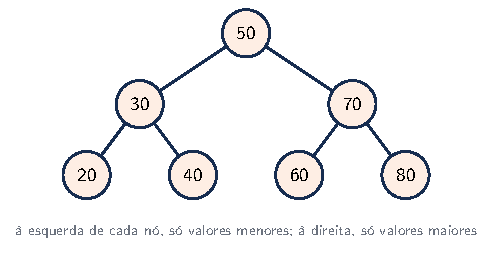
\includegraphics[width=0.62\linewidth,keepaspectratio]{imagens/capitulo-05_abb.pdf}
\end{center}

\subsubsection{Buscar}

Para procurar o 60 na árvore acima, compare com a raiz: 60 é maior que 50, então ele só pode estar à direita. Agora compare com o 70: 60 é menor, então desça à esquerda. Achou. Foram três comparações, e a metade esquerda da árvore nem foi olhada. É a mesma ideia da \textbf{busca binária} em um vetor ordenado, que você verá no Capítulo 7, só que agora em uma estrutura que aceita inserções e remoções.

\begin{codigo}
\begin{Verbatim}[breaklines=true, breaksymbolleft={}, fontsize=\footnotesize]
// trecho
    bool contem(int valor) const {
        No *atual = raiz;
        while (atual != nullptr) {
            if (valor == atual->valor) return true;
            atual = (valor < atual->valor) ? atual->esquerda : atual->direita;
        }
        return false;
    }
\end{Verbatim}
\end{codigo}

O \textbf{menor} valor da árvore é o nó mais à esquerda, e o \textbf{maior} é o nó mais à direita: basta descer sempre para o mesmo lado até não haver mais filho.

\subsubsection{Inserir}

Inserir é buscar o lugar onde o valor deveria estar. Quando a busca chega a um ponteiro nulo, é ali que o novo nó entra, sempre como \textbf{folha}. A versão recursiva fica curta: ela recebe a raiz de uma subárvore, insere o valor do lado certo e devolve a raiz, que muda apenas quando a subárvore estava vazia.

\begin{codigo}
\begin{Verbatim}[breaklines=true, breaksymbolleft={}, fontsize=\footnotesize]
// trecho
    static No *inserir(No *no, int valor) {
        if (no == nullptr) {
            return new No{valor};           // achou o lugar: nova folha
        }
        if (valor < no->valor) {
            no->esquerda = inserir(no->esquerda, valor);
        } else if (valor > no->valor) {
            no->direita = inserir(no->direita, valor);
        }
        // valor igual: já está na árvore, nada a fazer
        return no;
    }
\end{Verbatim}
\end{codigo}

A linha \texttt{no->esquerda = inserir(no->esquerda, valor)} é o truque que evita casos especiais: ela reconecta o filho, quer ele tenha mudado (era nulo e virou o nó novo), quer não. Esta implementação não guarda valores repetidos; quando for preciso, cada nó pode ter um contador de ocorrências.

\subsubsection{Percorrer em ordem}

Pela regra da ABB, o percurso em ordem visita primeiro todos os menores, depois o nó, depois todos os maiores. O resultado é que ele imprime os valores \textbf{ordenados}. Na árvore da figura: \texttt{20 30 40 50 60 70 80}. Uma ABB, portanto, é também uma forma de manter dados sempre em ordem.

\subsubsection{Remover}

A remoção é a operação mais delicada, porque o nó removido pode ter filhos que precisam continuar na árvore. Há três casos:

\begin{enumerate}
  \item \textbf{O nó é uma folha.} Basta apagá-lo e deixar nulo o ponteiro do pai.
  \item \textbf{O nó tem um filho.} O filho ocupa o lugar dele: o pai passa a apontar diretamente para o neto. A regra da ABB continua valendo, porque toda a subárvore do filho estava do mesmo lado do pai.
  \item \textbf{O nó tem dois filhos.} Nenhum dos filhos pode simplesmente subir, pois o outro ficaria sem lugar. A solução é encontrar o \textbf{sucessor}: o menor valor da subárvore direita. Ele é maior que tudo à esquerda e menor que todo o resto à direita, então pode ocupar o lugar do nó removido. Copiamos o valor do sucessor para o nó e removemos o sucessor lá de baixo, o que cai no caso 1 ou 2, já que o sucessor não tem filho à esquerda.
\end{enumerate}

\begin{center}
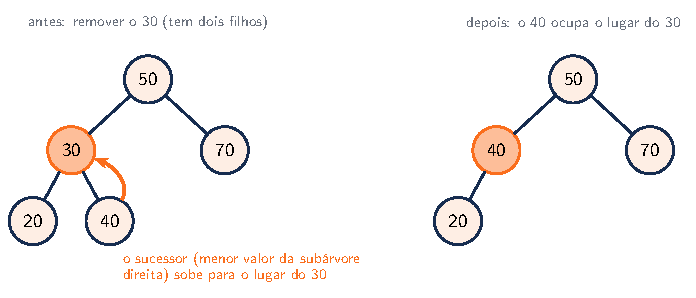
\includegraphics[width=0.85\linewidth,keepaspectratio]{imagens/capitulo-05_remocao.pdf}
\end{center}

\begin{codigo}
\begin{Verbatim}[breaklines=true, breaksymbolleft={}, fontsize=\footnotesize]
// trecho
    static No *remover(No *no, int valor) {
        if (no == nullptr) {
            return nullptr;                 // o valor não está na árvore
        }
        if (valor < no->valor) {
            no->esquerda = remover(no->esquerda, valor);
        } else if (valor > no->valor) {
            no->direita = remover(no->direita, valor);
        } else if (no->esquerda == nullptr) {   // casos 1 e 2: no máximo um filho
            No *filho = no->direita;
            delete no;
            return filho;
        } else if (no->direita == nullptr) {
            No *filho = no->esquerda;
            delete no;
            return filho;
        } else {                                // caso 3: dois filhos
            No *sucessor = no->direita;
            while (sucessor->esquerda != nullptr) {
                sucessor = sucessor->esquerda;
            }
            no->valor = sucessor->valor;        // o sucessor sobe
            no->direita = remover(no->direita, sucessor->valor);  // e sai lá de baixo
        }
        return no;
    }
\end{Verbatim}
\end{codigo}

Os casos 1 e 2 foram tratados juntos: se não há filho à esquerda, quem sobe é o da direita, e se este também for nulo, o pai simplesmente recebe \texttt{nullptr}. O programa completo aparece no final da próxima seção.

\subsection{5.5 Árvores balanceadas e degeneradas}

Buscar, inserir e remover descem um único caminho da raiz até, no máximo, uma folha. O custo dessas operações é, então, $O(h)$, em que $h$ é a altura da árvore. A questão é: qual é a altura?

Depende da \textbf{ordem de inserção}. As mesmas cinco chaves podem formar árvores muito diferentes:

\begin{center}
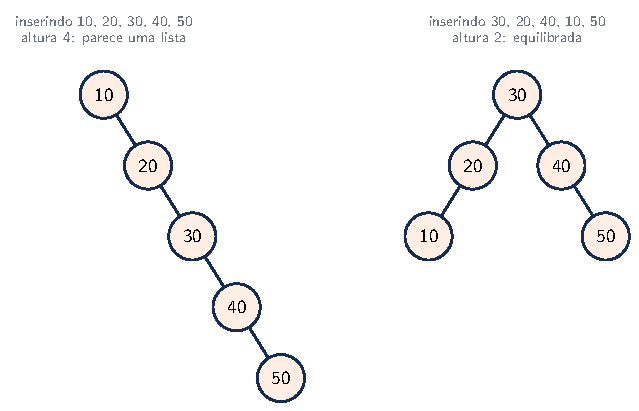
\includegraphics[width=0.8\linewidth,keepaspectratio]{imagens/capitulo-05_degenerada.pdf}
\end{center}

Quando os valores chegam já ordenados, cada novo nó vira filho direito do anterior, e a árvore \textbf{degenera} em algo igual a uma lista encadeada: altura $n - 1$ e busca $O(n)$. Quando a árvore está \textbf{balanceada}, isto é, com as subárvores de cada nó de alturas parecidas, a altura fica perto de $\log_2 n$, como você viu na conta da árvore cheia.

O experimento abaixo insere os números de 1 a 1000 de duas formas: em ordem crescente, e começando sempre pelo elemento do meio de cada intervalo:

\begin{codigo}
\begin{Verbatim}[breaklines=true, breaksymbolleft={}, fontsize=\footnotesize]
// trecho
void inserirDoMeio(ArvoreBusca &arvore, int inicio, int fim) {
    if (inicio > fim) return;
    int meio = (inicio + fim) / 2;
    arvore.inserir(meio);
    inserirDoMeio(arvore, inicio, meio - 1);
    inserirDoMeio(arvore, meio + 1, fim);
}

    ArvoreBusca crescente, equilibrada;
    for (int v = 1; v <= 1000; v++) {
        crescente.inserir(v);
    }
    inserirDoMeio(equilibrada, 1, 1000);
    cout << "Altura (crescente): " << crescente.altura() << endl;     // 999
    cout << "Altura (do meio): " << equilibrada.altura() << endl;     // 9
\end{Verbatim}
\end{codigo}

São os mesmos mil valores. Em uma árvore, achar o último exige percorrer mil nós; na outra, no máximo dez.

\begin{center}
\begin{tabular}{@{}p{0.26\linewidth}p{0.3\linewidth}p{0.3\linewidth}@{}}
\toprule
\rowcolor{headergray}
\tblheader{Operação} & \tblheader{ABB balanceada} & \tblheader{ABB degenerada} \\
\midrule
buscar & $O(\log n)$ & $O(n)$ \\
\rowcolor{rowgray} inserir & $O(\log n)$ & $O(n)$ \\
remover & $O(\log n)$ & $O(n)$ \\
\rowcolor{rowgray} mínimo e máximo & $O(\log n)$ & $O(n)$ \\
percorrer tudo & $O(n)$ & $O(n)$ \\
\bottomrule
\end{tabular}
\end{center}

Este é o programa completo da árvore binária de busca, com o experimento das alturas:

\begin{codigo}
\begin{Verbatim}[breaklines=true, breaksymbolleft={}, fontsize=\footnotesize]
#include <algorithm>   // max
#include <stdexcept>   // runtime_error

class ArvoreBusca {
private:
    struct No {
        int valor;
        No *esquerda = nullptr;
        No *direita = nullptr;
    };
    No *raiz = nullptr;

    static No *inserir(No *no, int valor) {
        if (no == nullptr) {
            return new No{valor};           // achou o lugar: nova folha
        }
        if (valor < no->valor) {
            no->esquerda = inserir(no->esquerda, valor);
        } else if (valor > no->valor) {
            no->direita = inserir(no->direita, valor);
        }
        // valor igual: já está na árvore, nada a fazer
        return no;
    }

    static No *remover(No *no, int valor) {
        if (no == nullptr) {
            return nullptr;                 // o valor não está na árvore
        }
        if (valor < no->valor) {
            no->esquerda = remover(no->esquerda, valor);
        } else if (valor > no->valor) {
            no->direita = remover(no->direita, valor);
        } else if (no->esquerda == nullptr) {   // casos 1 e 2: no máximo um filho
            No *filho = no->direita;
            delete no;
            return filho;
        } else if (no->direita == nullptr) {
            No *filho = no->esquerda;
            delete no;
            return filho;
        } else {                                // caso 3: dois filhos
            No *sucessor = no->direita;
            while (sucessor->esquerda != nullptr) {
                sucessor = sucessor->esquerda;
            }
            no->valor = sucessor->valor;        // o sucessor sobe
            no->direita = remover(no->direita, sucessor->valor);  // e sai lá de baixo
        }
        return no;
    }

    static void emOrdem(No *no) {
        if (no == nullptr) return;
        emOrdem(no->esquerda);
        cout << no->valor << " ";
        emOrdem(no->direita);
    }

    static int altura(No *no) {
        if (no == nullptr) return -1;
        return 1 + max(altura(no->esquerda), altura(no->direita));
    }

    static void liberar(No *no) {
        if (no == nullptr) return;
        liberar(no->esquerda);
        liberar(no->direita);
        delete no;
    }

public:
    ArvoreBusca() = default;
    ~ArvoreBusca() { liberar(raiz); }
    ArvoreBusca(const ArvoreBusca &) = delete;
    ArvoreBusca &operator=(const ArvoreBusca &) = delete;

    void inserir(int valor) { raiz = inserir(raiz, valor); }
    void remover(int valor) { raiz = remover(raiz, valor); }

    bool contem(int valor) const {
        No *atual = raiz;
        while (atual != nullptr) {
            if (valor == atual->valor) return true;
            atual = (valor < atual->valor) ? atual->esquerda : atual->direita;
        }
        return false;
    }

    int minimo() const {
        if (raiz == nullptr) throw runtime_error("árvore vazia");
        No *atual = raiz;
        while (atual->esquerda != nullptr) atual = atual->esquerda;
        return atual->valor;
    }

    int maximo() const {
        if (raiz == nullptr) throw runtime_error("árvore vazia");
        No *atual = raiz;
        while (atual->direita != nullptr) atual = atual->direita;
        return atual->valor;
    }

    int altura() const { return altura(raiz); }
    void imprimir() const { emOrdem(raiz); cout << endl; }
};

void inserirDoMeio(ArvoreBusca &arvore, int inicio, int fim) {
    if (inicio > fim) return;
    int meio = (inicio + fim) / 2;
    arvore.inserir(meio);
    inserirDoMeio(arvore, inicio, meio - 1);
    inserirDoMeio(arvore, meio + 1, fim);
}

int main() {
    ArvoreBusca arvore;
    for (int v : {50, 30, 70, 20, 40, 60, 80}) {
        arvore.inserir(v);
    }
    arvore.imprimir();                                   // 20 30 40 50 60 70 80
    cout << boolalpha << arvore.contem(60) << endl;      // true
    cout << arvore.contem(65) << endl;                   // false
    cout << arvore.minimo() << " " << arvore.maximo() << endl;  // 20 80
    cout << "Altura: " << arvore.altura() << endl;       // 2

    arvore.remover(30);   // dois filhos: o sucessor 40 sobe
    arvore.remover(40);   // agora o 40 tem um filho só, o 20
    arvore.remover(80);   // folha
    arvore.imprimir();                                   // 20 50 60 70

    ArvoreBusca crescente, equilibrada;
    for (int v = 1; v <= 1000; v++) {
        crescente.inserir(v);
    }
    inserirDoMeio(equilibrada, 1, 1000);
    cout << "Altura (crescente): " << crescente.altura() << endl;     // 999
    cout << "Altura (do meio): " << equilibrada.altura() << endl;     // 9
}
\end{Verbatim}
\end{codigo}

As funções recursivas ficaram \texttt{private} e \texttt{static}: quem usa a classe chama \texttt{inserir(valor)} sem precisar saber que existem nós, e a versão interna recebe a subárvore em que deve trabalhar. É o mesmo encapsulamento da pilha e da fila do Capítulo 4.

\subsection{5.6 Árvores AVL}

Na prática, você raramente controla a ordem em que os dados chegam. Cadastros por data, códigos sequenciais e nomes já ordenados são comuns, e são justamente o pior caso da ABB. A solução é uma árvore que \textbf{se rebalanceia sozinha} a cada inserção. A primeira delas, e a mais conhecida, é a \textbf{árvore AVL}, nome que vem das iniciais de seus criadores, Adelson-Velsky e Landis.

\subsubsection{Fator de balanceamento}

Cada nó da AVL guarda a própria altura. Com ela, calcula-se o \textbf{fator de balanceamento}:

\[ \text{fator} = \text{altura da subárvore esquerda} - \text{altura da subárvore direita} \]

A AVL exige que, em \textbf{todos} os nós, o fator seja $-1$, $0$ ou $+1$. Fator $+2$ significa que o nó pesa demais à esquerda; $-2$, que pesa demais à direita. Essa regra garante que a altura da AVL nunca passa de cerca de $1{,}44 \log_2 n$, então todas as operações ficam em $O(\log n)$.

\subsubsection{Rotações}

Quando uma inserção deixa algum nó com fator $\pm 2$, a árvore é consertada com uma \textbf{rotação}: uma troca de poucos ponteiros que faz um filho subir e o pai descer, \textbf{mantendo a regra da ABB}.

\begin{center}
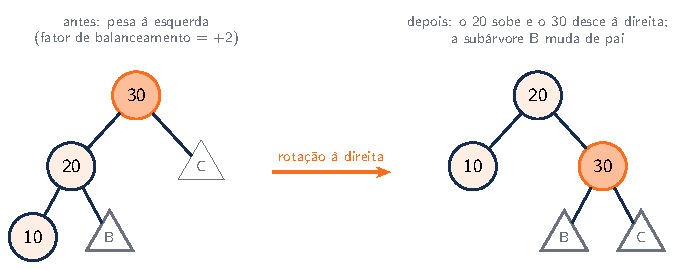
\includegraphics[width=0.85\linewidth,keepaspectratio]{imagens/capitulo-05_rotacao.pdf}
\end{center}

Na rotação à direita da figura, o 20 sobe e o 30 vira seu filho direito. A subárvore B, que estava à direita do 20, tem valores entre 20 e 30; por isso ela passa a ficar à esquerda do 30, e a ordem continua correta. A rotação à esquerda é o espelho dessa.

Há quatro situações de desequilíbrio, nomeadas pelo caminho do nó desequilibrado até o ponto onde entrou o novo valor:

\begin{center}
\begin{tabular}{@{}p{0.24\linewidth}p{0.3\linewidth}p{0.38\linewidth}@{}}
\toprule
\rowcolor{headergray}
\tblheader{Caso} & \tblheader{Como identificar} & \tblheader{Correção} \\
\midrule
esquerda-esquerda & fator $+2$, filho esquerdo com fator $\ge 0$ & rotação simples à direita \\
\rowcolor{rowgray} direita-direita & fator $-2$, filho direito com fator $\le 0$ & rotação simples à esquerda \\
esquerda-direita & fator $+2$, filho esquerdo com fator $-1$ & rotação dupla: à esquerda no filho, depois à direita no nó \\
\rowcolor{rowgray} direita-esquerda & fator $-2$, filho direito com fator $+1$ & rotação dupla: à direita no filho, depois à esquerda no nó \\
\bottomrule
\end{tabular}
\end{center}

Nos casos ``em linha'' (esquerda-esquerda e direita-direita), uma rotação basta. Nos casos ``em zigue-zague'', a primeira rotação endireita o zigue-zague, transformando-o no caso em linha, e a segunda resolve. Por exemplo, ao inserir 30, 10 e 20, o 20 entra à direita do 10, que está à esquerda do 30: é o caso esquerda-direita, e o resultado final tem o 20 na raiz.

\subsubsection{Inserção na AVL}

A inserção é a mesma da ABB, com um passo a mais: na volta da recursão, cada nó do caminho atualiza sua altura e, se precisar, é rebalanceado. Como a recursão volta de baixo para cima, o primeiro nó desequilibrado encontrado é o mais próximo da inserção, que é exatamente o que deve ser corrigido.

\begin{codigo}
\begin{Verbatim}[breaklines=true, breaksymbolleft={}, fontsize=\footnotesize]
#include <algorithm>   // max

struct NoAVL {
    int valor;
    int altura = 0;                // uma folha tem altura 0
    NoAVL *esquerda = nullptr;
    NoAVL *direita = nullptr;
};

int altura(NoAVL *no) { return no == nullptr ? -1 : no->altura; }

int fator(NoAVL *no) { return altura(no->esquerda) - altura(no->direita); }

void atualizar(NoAVL *no) {
    no->altura = 1 + max(altura(no->esquerda), altura(no->direita));
}

NoAVL *rotacaoDireita(NoAVL *y) {
    NoAVL *x = y->esquerda;
    NoAVL *b = x->direita;
    x->direita = y;                // y desce para a direita de x
    y->esquerda = b;               // a subárvore B muda de pai
    atualizar(y);                  // y primeiro, porque agora está embaixo
    atualizar(x);
    return x;                      // x é a nova raiz desta subárvore
}

NoAVL *rotacaoEsquerda(NoAVL *x) {
    NoAVL *y = x->direita;
    NoAVL *b = y->esquerda;
    y->esquerda = x;
    x->direita = b;
    atualizar(x);
    atualizar(y);
    return y;
}

NoAVL *balancear(NoAVL *no) {
    atualizar(no);
    int f = fator(no);
    if (f > 1) {                                   // pesa à esquerda
        if (fator(no->esquerda) < 0) {             // zigue-zague: esquerda-direita
            no->esquerda = rotacaoEsquerda(no->esquerda);
        }
        return rotacaoDireita(no);
    }
    if (f < -1) {                                  // pesa à direita
        if (fator(no->direita) > 0) {              // zigue-zague: direita-esquerda
            no->direita = rotacaoDireita(no->direita);
        }
        return rotacaoEsquerda(no);
    }
    return no;                                     // já está equilibrado
}

NoAVL *inserir(NoAVL *no, int valor) {
    if (no == nullptr) return new NoAVL{valor};
    if (valor < no->valor) {
        no->esquerda = inserir(no->esquerda, valor);
    } else if (valor > no->valor) {
        no->direita = inserir(no->direita, valor);
    } else {
        return no;                                 // repetido: nada muda
    }
    return balancear(no);                          // conserta na volta da recursão
}

void preOrdem(NoAVL *no) {
    if (no == nullptr) return;
    cout << no->valor << " ";
    preOrdem(no->esquerda);
    preOrdem(no->direita);
}

void liberar(NoAVL *no) {
    if (no == nullptr) return;
    liberar(no->esquerda);
    liberar(no->direita);
    delete no;
}

int main() {
    NoAVL *raiz = nullptr;
    for (int v : {30, 10, 20}) {                   // caso esquerda-direita
        raiz = inserir(raiz, v);
    }
    preOrdem(raiz); cout << endl;                  // 20 10 30
    liberar(raiz);

    raiz = nullptr;
    for (int v = 1; v <= 7; v++) {                 // em ordem crescente
        raiz = inserir(raiz, v);
    }
    preOrdem(raiz); cout << endl;                  // 4 2 1 3 6 5 7
    cout << "Altura: " << altura(raiz) << endl;    // 2
    liberar(raiz);

    raiz = nullptr;
    for (int v = 1; v <= 1000; v++) {
        raiz = inserir(raiz, v);
    }
    cout << "Altura com 1000: " << altura(raiz) << endl;   // 9
    liberar(raiz);
}
\end{Verbatim}
\end{codigo}

Inserir de 1 a 7 em ordem crescente, que na ABB comum produziria uma ``lista'' de altura 6, gera na AVL uma árvore cheia de altura 2, com o 4 na raiz. E os mil valores crescentes, que deixaram a ABB com altura 999, ficam com altura 9. Cada rotação custa $O(1)$, pois mexe em poucos ponteiros, e há no máximo uma correção (simples ou dupla) por inserção; o custo total continua $O(\log n)$.

A remoção na AVL segue a mesma ideia: remove-se como na ABB e chama-se \texttt{balancear} na volta da recursão. A diferença é que, na remoção, pode ser preciso rebalancear vários nós no caminho até a raiz.

\begin{destaque}{Outras árvores balanceadas}
A AVL não é a única. A \textbf{árvore rubro-negra} (\textit{red-black tree}) usa uma regra mais folgada, baseada em cores nos nós, e faz menos rotações nas inserções e remoções; ela é a base do \texttt{std::set} e do \texttt{std::map} do C++. Já as \textbf{árvores B} têm nós com muitos filhos e são usadas em bancos de dados e sistemas de arquivos, em que cada nó corresponde a um bloco do disco.
\end{destaque}

\subsection{5.7 Árvores prontas}

Em projetos reais, você usará as árvores balanceadas da biblioteca padrão. O \texttt{std::set} guarda valores sem repetição e o \texttt{std::map} guarda pares chave-valor; ambos mantêm os elementos \textbf{ordenados} e fazem inserção, busca e remoção em $O(\log n)$.

\begin{codigo}
\begin{Verbatim}[breaklines=true, breaksymbolleft={}, fontsize=\footnotesize]
#include <set>
#include <map>

int main() {
    set<int> numeros = {50, 30, 70, 20, 40};
    numeros.insert(60);
    numeros.insert(30);                     // repetido: ignorado
    numeros.erase(70);
    for (int n : numeros) {
        cout << n << " ";                   // sempre em ordem
    }
    cout << endl;                           // 20 30 40 50 60
    cout << numeros.count(40) << endl;      // 1: está no conjunto

    map<string, int> idades;
    idades["Caio"] = 20;
    idades["Ana"] = 19;
    idades["Bia"] = 21;
    for (const auto &[nome, idade] : idades) {
        cout << nome << ": " << idade << endl;  // Ana: 19, Bia: 21, Caio: 20
    }
}
\end{Verbatim}
\end{codigo}

\begin{destaque}{Comparando com Python}
Python não tem uma árvore de busca na biblioteca padrão. O \texttt{dict} e o \texttt{set} usam \textbf{tabelas hash}, que buscam em $O(1)$ em média, mas não guardam as chaves em ordem: para percorrê-las ordenadas, é preciso chamar \texttt{sorted}, que custa $O(n \log n)$ a cada vez. Quando a ordem importa, você pode escrever sua própria árvore, e o código fica parecido com o do C++, sem ponteiros explícitos nem \texttt{delete}, porque o coletor de lixo libera os nós:

\begin{codigo}
\begin{Verbatim}[breaklines=true, breaksymbolleft={}, fontsize=\footnotesize]
class No:
    def __init__(self, valor):
        self.valor = valor
        self.esquerda = None
        self.direita = None

def inserir(no, valor):
    if no is None:
        return No(valor)
    if valor < no.valor:
        no.esquerda = inserir(no.esquerda, valor)
    elif valor > no.valor:
        no.direita = inserir(no.direita, valor)
    return no

def em_ordem(no):
    if no is not None:
        yield from em_ordem(no.esquerda)
        yield no.valor
        yield from em_ordem(no.direita)

raiz = None
for v in [50, 30, 70, 20, 40]:
    raiz = inserir(raiz, v)
print(list(em_ordem(raiz)))    # [20, 30, 40, 50, 70]
\end{Verbatim}
\end{codigo}
\end{destaque}

\subsection{Erros Comuns}

\begin{itemize}
  \item \textbf{Esquecer o caso da árvore vazia.} Toda função recursiva sobre árvores precisa começar testando \texttt{nullptr}. Sem isso, a recursão acessa um ponteiro nulo ao chegar abaixo de uma folha.
  \item \textbf{Não reconectar o filho na inserção recursiva.} Chamar apenas \texttt{inserir(no->esquerda, valor)}, sem atribuir o resultado a \texttt{no->esquerda}, cria o nó novo e o perde: ele nunca é ligado à árvore e a memória vaza.
  \item \textbf{Liberar o pai antes dos filhos.} Depois do \texttt{delete} de um nó, seus ponteiros não podem mais ser lidos. Libere sempre em pós-ordem.
  \item \textbf{Conferir a regra da ABB só com os filhos diretos.} A regra vale para a subárvore inteira: um valor 55 na subárvore esquerda do 50 quebra a árvore, mesmo que ele seja menor que o pai imediato.
  \item \textbf{Escolher o sucessor errado na remoção.} O sucessor é o \textit{menor} valor da subárvore \textit{direita} (desça uma vez à direita e depois sempre à esquerda). Também funciona usar o \textit{maior} da subárvore esquerda, mas não misture as duas ideias.
  \item \textbf{Supor que a ABB é sempre $O(\log n)$.} Isso só vale se ela estiver balanceada. Com dados ordenados, uma ABB comum vira uma lista.
  \item \textbf{Atualizar as alturas na ordem errada na rotação.} O nó que desceu deve ser atualizado antes do que subiu, porque a altura do novo pai depende da altura do novo filho.
  \item \textbf{Esperar ordem do \texttt{dict} ou do \texttt{set} do Python.} O \texttt{dict} preserva a ordem de inserção, não a ordem das chaves, e o \texttt{set} não garante ordem nenhuma.
\end{itemize}
